\documentclass{article}
\usepackage{graphicx}
\usepackage{array}
\usepackage{amsmath}
\usepackage{caption}
\usepackage{subcaption}
\usepackage{booktabs}
\usepackage{changepage}
\usepackage{titling}
\usepackage{tikz}
\usepackage{pgfplots}
\usepackage{xcolor}
\usepackage[a4paper, total={6in,9in}]{geometry}

\usetikzlibrary{calc,patterns,angles,quotes}
\captionsetup[table]{name=\textit{Tabella}}
\renewcommand\maketitlehooka{\null\mbox{}\vfill}
\renewcommand\maketitlehookd{\vfill\null}
\renewcommand*\contentsname{Indice}
\pgfplotsset{compat=1.18}

\title{Esperienza 0 - Pendolo di Kater}
\author{Matteo Herz}
\date{7 Gennaio 2024}

\begin{document}
\begin{titlepage}
	\begin{center}
		\vspace*{1cm}
		
		\textbf{\huge Relazione Pendolo di Kater}
		
		\vspace{0.6cm}
		{\LARGE Matteo Herz} \\
		\vspace{0.5cm}
		{\large 7 Gennaio 2024}
		\vspace{3cm}
		
		\begin{tikzpicture}[scale=2.0]
			% save length of g-vector and theta to macros
			\pgfmathsetmacro{\Gvec}{1.5}
			\pgfmathsetmacro{\myAngle}{30}
			% calculate lengths of vector components
			\pgfmathsetmacro{\Gcos}{\Gvec*cos(\myAngle)}
			\pgfmathsetmacro{\Gsin}{\Gvec*sin(\myAngle)}
			
			\coordinate (centro) at (0,0);
			\draw[dashed,gray,-] (centro) -- ++ (0,-3.5) node (mary) [black,below]{$ $};
			\draw[thick] (centro) -- ++(270+\myAngle:3) coordinate (bob);
			\pic [draw, ->, "$\theta$", angle eccentricity=1.5] {angle = mary--centro--bob};
			\draw [blue,-stealth] (bob) -- ($(bob)!\Gcos cm!(centro)$);
			\draw [-stealth] (bob) -- ($(bob)!-\Gcos cm!(centro)$)
			coordinate (gcos)
			node[midway,above right] {$a\cos\theta$};
			\draw [-stealth] (bob) -- ($(bob)!\Gsin cm!90:(centro)$)
			coordinate (gsin)
			node[midway,above left] {$a\sin\theta$};
			\draw [-stealth] (bob) -- ++(0,-\Gvec)
			coordinate (g)
			node[near end,left] {$g$};
			\pic [draw, ->, "$\theta$", angle eccentricity=1.5] {angle = g--bob--gcos};
			\filldraw [fill=black!40,draw=black] (bob) circle[radius=0.1];
		\end{tikzpicture}
		
		\vfill   %riempie in verticale fino a fine pagina 
		
		\vspace{0.8cm}
		
		Università degli studi di Torino\\
		Laurea Triennale in Fisica\\
		\vspace*{0.1cm}
		
		
	\end{center}
\end{titlepage}

\newpage

\tableofcontents 

\newpage 
\section{Scopo dell'esperienza}
L'esperienza di laboratorio consiste nel valutare da un punto di vista fisico-statistico la qualità di 100 misurazioni del periodo di oscillazione di un pendolo reversibile (chiamato \textit{Pendolo di Kater}). 

Tale valutazione si basa sull'utilizzo di test statistici in grado di stimare quanto le misurazioni effettuate siano affette o meno da errori sistematici, la cui presenza indirizzerebbe inevitabilmente il risultato verso valori non compatibili (entro soglie fissate) con il valore vero del periodo di oscillazione. \\

Lungo tutto l'arco della descrizione dell'esperienza di laboratorio farò riferimento al valore vero, indicato con la lettera $\mu$, come all'effettivo valore del periodo di oscillazione del pendolo di Kater, calcolato sperimentalmente con una fotocellula avente una sensibilità di un millesimo di secondo.

\section{Strumentazione utilizzata}

\begin{table}[ht]
	\centering
	\captionof{table}{\textit{Strumenti e relative sensibilità}}
	\begin{tabular}{@{}lc@{}}
		\toprule
		\textbf{Strumento} & \textbf{Sensibilità strumento} \\
		\midrule
		Fotocellula & 0.001 s \\
		Cronometro digitale & 0.01 s \\
		Pendolo di Kater & - \\
		\bottomrule
	\end{tabular}
\end{table}

\section{Procedura di misura effettuata}
Le misurazioni sono state effettuate a casa attraverso un cronometro digitale dalla sensibilità di 0.01 s.
In particolare le 100 misure sono state ottenute tutte una di fila all'altra, guardando un video preregistrato del pendolo in fase di oscillazione.

\section{Analisi Dati}

\hspace{0.6cm}
    \begin{minipage}[c]{0.45\textwidth}
    	\centering 
        \captionof{table}{\textit{Dati non accorpati}}
        \begin{tabular}{llrr}
        	\toprule
            Media & $\bar{x}$ & 1.95 & s \\
            Varianza & $\sigma^2_x$ & 0.0070 & $s^2$ \\
            Dev. std & $\sigma_x$ & 0.083 & s \\
            Dev. std (media) & $\sigma_{\bar{x}}$ & 0.0083 & s \\
            Mediana & \textit{Me} & 1.95 & s \\
            Moda & $\tilde{x}$ & 1.94 & s \\
            \bottomrule 
        \end{tabular}
    \end{minipage}%
    \begin{minipage}[c]{0.45\textwidth}
    	\centering
        \captionof{table}{\textit{Dati accorpati}}
        \begin{tabular}{llrr}
        	\toprule
            Media & $\bar{x}$ & 1.95 & s \\
            Varianza & $\sigma^2_x$ & 0.0068 & $s^2$ \\
            Dev. std & $\sigma_x$ & 0.082 & s \\
            Dev. std (media) & $\sigma_{\bar{x}}$ & 0.0083 & s \\
            Mediana & \textit{Me} & - & - \\
            Moda & $\tilde{x}$ & - & - \\
            \bottomrule
        \end{tabular}
    \end{minipage}
    \vspace{0.4cm}

\noindent
Come si evince dal confronto dei dati delle tabelle sopra riportate, l'accorpamento dei dati non ha portato a significativi cambiamenti nei rispettivi campi.
\begin{table}[ht]
\centering
\captionof{table}{\textit{Dati prima e dopo l'accorpamento con variazioni percentuali}}
\begin{tabular}{lcccc}
\toprule
\textbf{Statistica} & \textbf{Simbolo} & \textbf{Valore Prima} & \textbf{Valore Dopo} & \textbf{Variazione Percentuale} \\
\midrule
Media & $\bar{x}$ & 1.95 s & 1.95 s & 0\% \\
Varianza & $\sigma^2$ & 0.0070 s² & 0.0068 s² & -2.86\% \\
Dev. std & $\sigma_x$ & 0.083 s & 0.082 s & -1.20\% \\
Dev. std (media) & $\sigma_{\bar{x}}$ & 0.0083 s & 0.0083 s & 0\% \\
\bottomrule
\end{tabular}
\label{tab:dati_accorpati}
\end{table}

\subsection{Test del 3-$\sigma_{x}$ }
Prima di procedere all'accorpamento dei dati ho effettuato quello che abbiamo definito come \textit{Test del 3-$\sigma$}. Questo test permette di determinare se una data misurazione all'interno del nostro campione sia eliminabile o meno. Per fare ciò mi baso sulla probabilità empirica legata alla distrubuzione di Gauss di osservare il dato in questione.
\newline\indent
Se la probabilità di osservare tale misura (\textit{t}) risulta minore della probabilità di osservare misure più distanti di 3 deviazioni standard $\sigma_x$ dal valore centrale $\bar{x}$, ovvero $P( |t| > \mu - 3\sigma_{x}) \approx 0.3\% $, e tenendo conto che nel nostro caso su 100 misurazioni questo corrisponderebbe ad osservarne meno di una, allora quest'ultima può essere considerata "estranea" al campione di popolazione preso in analisi e dunque rigettata.
\newline\newline 
Applicando il test del 3-$\sigma_x$ ai 100 dati ottenuti, mi trovo a dover rigettare un misura, pari a 2.21 s.
\\Tale misura eccede di 0.01 s oltre il valore soglia di $\bar{x}$ + 3$\sigma_x$, corrispondente a 2.20 s.

Dunque, d'ora in avanti avrò $N = 99$. 

\subsection{Errore sulla stima - Sensibilità dello strumento}
Il confronto tra la deviazione standard della media (considerata come errore sulla stima) e la sensibilità dello strumento indica che l'incertezza nei dati raccolti è circa minore del 17\% rispetto alla sensibilità dello strumento. Questo suggerisce che, pur essendoci una certa variabilità nei dati, questa variabilità risulta essere ancora contenuta entro i limiti di precisione del nostro strumento. Sulla base di queste osservazioni posso dedurre che i dati generati dall'esperimento siano abbastanza precisi in relazione alla sensibilità dello strumento utilizzato.

\subsection{Risultato ottenuto}
In definitiva, la stima del periodo di oscillazione del pendolo ottenuta dall'analisi dati risulta essere: 
\begin{center}
$\mathbf{1.95 \pm 0.01 \, \text{s}}$
\end{center}

\section{Test del $\chi^2$}
A fronte dell'esperienza condotta, mi aspetto che a descrivere l'istogramma sperimentale delle misure ripetute del periodo di oscillazione del pendolo sia la \textit{distribuzione di Gauss}.

Questo poiché suppongo che le misurazioni effettuate siano soggette principalmente a sorgenti di errori casuali e trascurabili errori sistematici. Se così dovesse risultare, i valori misurati sarebbero distribuiti su una curva a campana centrata attorno alla miglior stima del valore vero $\bar{x}$, non distante da $\mu$. 
Nel caso in cui invece fossimo in presenza di errori sistematici non trascurabili dovrei osservare la distribuzione limite centrata su un valore $\bar{x}$ distante dal valor vero $\mu$ calcolato dalla fotocellula.

\subsection{Istogramma delle frequenze}

\vspace{0.3cm}
\begin{center}
	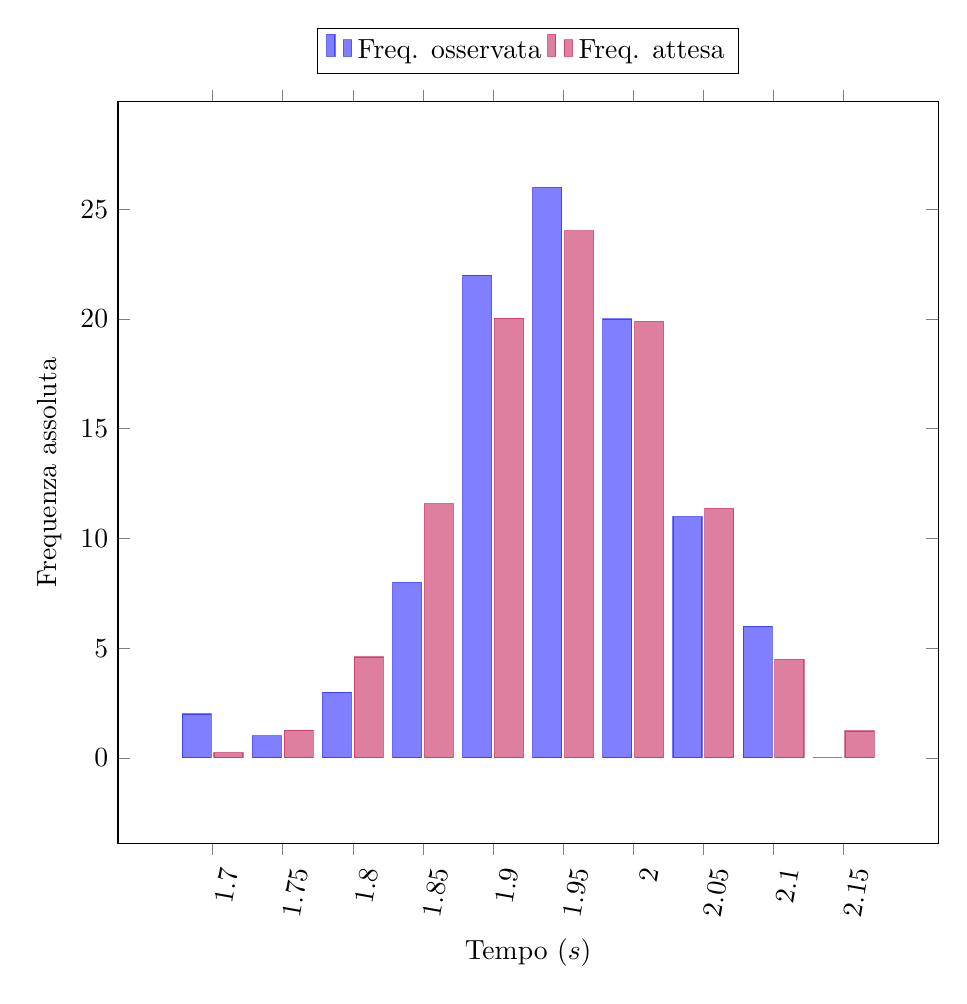
\begin{tikzpicture}
		\pgfplotsset{compat = 1.3}
		\begin{axis}[
			width=12cm, 
			height=11cm,
			ylabel=Frequenza assoluta,
			xlabel=Tempo $(s)$,
			enlargelimits=0.15,
			legend style={at={(0.5,1.1)},	anchor=north,legend columns=-1},
			ybar= 1pt,% configures `bar shift'
			bar width=10.5pt,
			xtick={
				1.700,
				1.750,
				1.800,
				1.850,
				1.900,
				1.950,
				2.000,
				2.050,
				2.100,
				2.150},
			xticklabel style={rotate=80, anchor=north east}
			]
			\addplot+[opacity=0.5,color=blue] 
			coordinates {
				(1.700,2)
				(1.750,1)
				(1.800,3)
				(1.850,8)
				(1.900,22)
				(1.950,26)
				(2.000,20)
				(2.050,11)
				(2.100,6)
				(2.150,0)};
			\addplot+[opacity=0.5, color=purple]
			coordinates {
				(1.700,0.240)
				(1.750,1.263)
				(1.800,4.600)
				(1.850,11.590)
				(1.900,20.040)
				(1.950,24.023)
				(2.000,19.891)
				(2.050,11.376)
				(2.100,4.494)
				(2.150,1.226)};
			\legend{Freq. osservata,Freq. attesa}
		\end{axis}
	\end{tikzpicture}
\end{center}
\vspace{0.2cm}

\subsection{Ipotesi del Test}
\begin{align*}
    &\text{$H_0$:} \text{ la distribuzione di Gauss si adatta alla distribuzione delle misure effetuate}     \\ \
	&\text{$H_1$:} \text{ la distribuzione di Gauss non si adatta alla distribuzione delle misure effettuate } \
\end{align*}

\subsection{Dati ottenuti}

\begin{table}[ht]
	\centering
	\begin{tabular}{@{}lc@{}}
		\toprule
		\textbf{Dati} & \textbf{Valori} \\
		\midrule
		Livello di significatività scelto ($\alpha $) & 0.05 \\
		Numero di gradi di libertà & 4 \\
		Valore del $\chi^2$ critico & 9.49 \\
		Valore del $\chi^2$ calcolato & 1.72 \\
		\bottomrule
	\end{tabular}
	\captionof{table}{\textit{Dati del test del $\chi^2$ per la verifica della distribuzione delle misure}}
\end{table}

\subsection{Conclusione Test del $\chi^2$}
L'ipotesi nulla ($H_0$) che la distribuzione di Gauss si adatti alla distribuzione delle misure effettuate è confermata dai dati calcolati. Il valore del $\chi^2$ calcolato, pari a 1.72, con 4 gradi di libertà, è inferiore al valore critico della variabile $\chi^2$ a un livello di significatività del 5\%, che risulta essere 9.49.

Inoltre si osserva che il $\chi^2$ calcolato è relativamente basso rispetto al valore critico, indicando un \textit{fit} coerente della distribuzione di Gauss a quella relativa alle 100 misurazioni. 
\\In conclusione, la distribuzione di Gauss può essere considerata compatibile con i dati raccolti.

\section{Test di Gauss}
\subsection{Stima del Periodo e Misura della Fotocellula}

La stima del periodo del pendolo calcolata ($\bar{x}$) e la stima teorica ($\mu$), con relative incertezze e unità di misura, risultano essere:
\begin{align*}
	\bar{x} = 1.95 &\pm 0.01\text{ s}\\ \
	\mu      = 1.957 &\pm 0.001 \text{ s} \
\end{align*}

\subsection{Test di Compatibilità tra le Misure}
Per verificare se $\bar{x}$ e $\mu$ sono compatibili, utilizzo il test di Gauss o "test z".

Il test viene eseguito prendendo per vera in partenza la cosiddetta "ipotesi nulla" ($H_0$), ovvero che i due valori siano effettivamene compatibili. Lo scopo del test è dunque quello di capire se l'ipotesi $H_0$ debba essere rigettata (confermando invece l'ipotesi $H_1$) o meno. \\

Per poter decretare la compatibilità o meno di $\bar{x}$ con $\mu$, il test prende in considerazione la distanza in valore assoluto di $\bar{x}$ con $\mu$, espressa in unità di deviazioni standard della media ($\sigma_{\bar{x}}$), ovvero la variabile $z_{oss}$, definita come segue: 

\[ z_{\text{oss}} = \frac{| \bar{x} - \mu |}{\sigma_{\bar{x}}} \]
\vspace{0.1 cm}

\noindent Il valore così ricavato ci permette di calcolare l'area alle code della gaussiana corrispondenti a discrepanze maggiori in valore assoluto di tale numero, ovvero $P( | z_i |> z_{oss} )$, per definizione la probabilità di osservare stime ($\bar{x}_i$) corrispondenti a discrepanze maggiori di $z_{oss}$ :
\vspace{0.2cm}

\[ \frac{1}{\sqrt{2\pi}} \bigg( \int_{-\infty}^{- z_{oss}}e^{-\frac{-z^2}{2}} \,dz +  \int_{z_{oss}}^{+ \infty}e^{-\frac{-z^2}{2}} \,dz \bigg)  \quad = \quad 1 - \bigg( \frac{1}{\sqrt{2\pi}} \int_{-z_{oss}}^{+ z_{oss}}e^{-\frac{-z^2}{2}} \,dz \bigg) \]
\vspace{0.2cm}

\noindent Il numero ottenuto è definito come il "p-value".\\
 Nel caso in cui il p-value calcolato risultasse maggiore di un certo \textit{livello di significatività} (indicato con $\alpha$), potremmo stabilire che $\bar{x}$ è effettivamente compatibile con $\mu$, e dunque affetta da errori sistematici trascurabili rispetto alle sole fluttuazioni statistiche.\\
	
In caso contrario invece ( p-value < $\alpha$ ), dovremmo dedurre che una tale discrepanza sia dovuta ad errori sistamatici non trascurabili, e dunque rigettare $H_0$.

\subsection{Ipotesi del Test}

\subsection{Dati ottenuti}

\begin{table}[ht]
    \centering
            \begin{tabular}{|l|c|p{10cm}|}
                \hline
                    \textbf{Voce} & \textbf{Descrizione} \\
                \hline
                    Ipotesi del test & \textbf{\(H_0\)}: I due valori sono compatibili \\
                \hline
                    Livello di significatività scelto ($\alpha$) & 0.05 \\
                \hline
                  p-value & 0.368 \\
                \hline 
                    Valore Critico della Variabile Statistica ($z_{critico}$)  &  1.96 \\
                \hline
                    Valore della Variabile Statistica Calcolata ($z_{oss}$) & 0.90 \\
                \hline          
            \end{tabular}
        \captionof{table}{\textit{Parametri del test di Gauss}}
        \label{tab:gauss_test}
\end{table}

\subsection{Conclusione del Test}
Il valore della variabile statistica calcolata è inferiore al valore critico, e il p-value è superiore al livello di significatività, dunque possiamo confermare l'ipotesi nulla ($H_0$) di compatibilità tra la stima del periodo di oscillazione $\bar{x} = 1.95 \pm 0.01 \text{ s}$ e la media della popolazione (valor vero) $\mu = 1.957 \pm 0.001 \text{ s}$, il tutto con un livello di significatività $\alpha = 5\%$.

Tale compatibilità indica che siamo effetivamente in presenza di errori sistematici trascurabili rispetto agli errori casuali (fluttuazioni statistiche).

\subsection{Commenti}
\begin{itemize}
    \item \textbf{Analisi degli Errori:} \textit{L'analisi degli errori suggerisce miglioramenti nella procedura di misurazione o negli strumenti utilizzati per futuri esperimenti?}
    
    Sicuramente una misurazione del periodo di oscillazione del pendolo di Kater effettuata dal vivo potrebbe risultare più precisa rispetto ad un misurazione effettuata via video, con schermi aventi talvolta frequenze di aggiornamento e latenze differenti.
    
    Inoltre l'utilizzo di cronometri aventi sensibilità di 0.01 s limita in parte l'analisi dati costringendoci a considerare meno cifre significative e a dover compiere alcune considerazioni come in [4.2]. 
    
    \item \textbf{Errori Sistematici:} \textit{Sono presenti errori sistematici? È possibile escluderli? Se non è possibile, quanto incidono rispetto agli errori casuali?}

    Sicuramente sono presente errori sistematici legati alla sensibilità non elevata (0.01 s) dei cronometri utilizzati, piuttosto che errori sistematici legati alla video registrazione e ai dispositivi su cui questa viene riprodotta, come citato sopra.
    
    Inoltre non è possibile escludere totalmente la presenza di errori sistematici in quanto fortemente legati, in maniera intrinseca, ai nostri strumenti di lavoro non professionali.
    \\Nonostante questo però, come emerge dall'analisi dati, questi ultimi incidono in maniera trascurabile rispetto alle fluttuazioni statistiche, presenti invece lungo tutta la procedura di misurazione.
    
\end{itemize}

\section{Intervalli $\mu \pm \sigma_x$ e $\mu \pm \sigma_{\bar{x}}$} 
\textbf{Intervallo} $\mu \pm \sigma_x$: rappresenta l'intervallo di confidenza del 68\% attorno alla media della popolazione ($\mu$), dove $\sigma_x$ è la deviazione standard delle singole misure. Questo significa che se si considera la deviazione standard come incertezza sulla singola misura (cioè $x = \mu \pm \sigma_x$), si può avere fiducia al 68\% che tale misura si trovi entro una deviazione standard dal valor vero.
\\\\ \noindent\textbf{Intervallo} $\mu \pm \sigma_{\bar{x}}$: rappresenta l'intervallo di confidenza del 68\% attorno alla media della popolazione ($\mu$), dove $\sigma_{\bar{x}}$ è la deviazione standard della media.
\\Se si compissero infatti molte determinazioni della media di $N$ misure, allora i risultati $\bar{x}$ si distribuirebbero attorno a $\mu$ con larghezza $\sigma_{\bar{x}} =  \frac{\sigma_x}{\sqrt{N}} $.
\\ Dunque, se si calcolasse la media di $N$ misure una volta, si potrebbe essere confidenti al 68\% che tale risultato giaccia entro una distanza $ \sigma_{\bar{x}}$ dal valor vero.

\subsection{$N$ misure necessarie}
Per determinare il numero di misure $N$ necessarie affinché l'errore sulla media sia uguale alla sensibilità dello strumento, utilizzo la formula per il calcolo dell'errore standard della media ($\sigma_{\bar{x}}$):

\[\sigma_{\bar{x}} = \frac{\sigma_x}{\sqrt{N}}\]

\noindent Dove:
\begin{itemize}
  \item $\sigma_{\bar{x}}$ è l'errore standard della media
  \item $\sigma_x$ è la deviazione standard delle singole misure
  \item $N$ è il numero di misure.
\end{itemize}

\noindent Dunque basta risolvere questa equazione rispetto a $N$ per ottenere il numero necessario di misure. \\Se la sensibilità dello strumento è $\delta$ e voglio che l'errore sulla media ($\sigma_{\bar{x}}$) sia uguale a $\delta$, allora risolverò l'equazione:

\[\frac{\sigma_x}{\sqrt{N}} = \delta\]

\noindent Risolvendo per $N$ ottengo:

\[N = \left( \frac{\sigma_x}{\delta} \right)^2\]

\noindent Sostituendo i valori numerici:

\[N \approx 68 \]

\section{Conclusione}
\subsection{Sintesi Quantitativa dei Risultati dell'Esperienza}

\begin{table}[ht]
	\centering
	\begin{tabular}{|l|r|r|c|}
		\hline
		\textbf{Test} & \textbf{Valori Ottenuti} & \textbf{Valori Limite} & \textbf{Esito}  \\
		\hline
		Test del $\chi^2$ & $\chi^2_{oss} = 1.72$  & $\chi^2_{critico} = 9.49$ &  Test Superato \\
		\hline
		Test di Gauss & $z_{oss} = 0.90$ & $z_{critico} = 1.96$ & Test Superato \\
		& $p-value_{oss} = 0.368$ & $ \alpha = 0.05$ &   \\
		\hline
	\end{tabular}
    \captionof{table}{\textit{Sintesi Quantitativa dei Risultati dell'Esperienza}}
\end{table}

\[ \text{\textbf{Media del Periodo di oscillazione \underline{calcolata}}  } \rightarrow \bar{x} = 1.95 \pm 0.01\text{ s} \]
\[ \quad\quad \text{\textbf{Media del Periodo di oscillazione \underline{teorica}}    } \rightarrow \mu = 1.957 \pm 0.001 \text{ s} \]

\subsection{Qualità della misura}
Al fronte dei risultati ottenuti e degli esiti dei test, le misure sono risultate precise e sufficientemente accurate, con un media ($\bar{x}$) calcolata distante 0.9 $\sigma_{\bar{x}}$ dal valor vero ($\mu$) registrato dalla fotocellula. 

Inoltre come evidenziato in [4.2], il confronto tra la deviazione standard della media e la sensibilità dello strumento suggerisce che i risultati ottenuti in fase di misurazione sono precisi rispetto alla sensibilità dello strumento utilizzato.

\subsection{Possibili fonti di errore}
\begin{itemize}
	\item \textbf{Errori sistematici:} Come citato in [6.6] possibili fonti di errori sistematici possono essere sorte sia dall'utilizzo di una strumentazione non professionale con sensibilità non elevate, piuttosto che da misure effettuate via video. Inoltre la sensibilità e la prontezza dei riflessi variano da persona a persona, a differenza della precisione di macchina di una fotocellula.
	
	Nonostante questo, come si evince dal test di Gauss e dal test del $\chi^2$ gli errori sistematici risultano trascurabili rispetto alle sole fluttuazioni statistiche.
	
	\item \textbf{Errori casuali:} Possibili fonti di errori casuali (fluttuazioni statistiche) sono dovute per lo più ai miei riflessi e alla prontezza in fase di misurazione, ma in secondo luogo anche ad altre possibili fonti esterne (ad esempio distrazioni).
	
	Come dimostrato dal test del $\chi^2$, gli errori sistematici risultano trascurabili rispetto ai soli errori casuali, la cui presenza nelle misurazioni denota proprio una distribuzione gaussiana limite in accordo con la distribuzione delle misure effettuate.

\end{itemize}

\subsection{Test condotti ed esiti}
\begin{enumerate}
	\item \textbf{Test di Gauss:} Il test di Gauss conferma l'ipotesi $H_0$ \textbf{confermando} (CAMBIARE) l'accordo tra la media  calcolata ($\bar{x}$) e la media della popolazione ($\mu$) calcolata attraverso la fotocellula.
	\item \textbf{Test del $\chi^2$:} Il test del $\chi^2$ conferma l'ipotesi $H_0$, \textbf{confermando} che la distribuzione normale attesa si adatta alla distribuzione dei dati osservati.
\end{enumerate}

\end{document}
https://www.overleaf.com/project/65870edfd7e2495b8821da45